%\documentclass{article}
\documentclass[journal]{IEEEtran}
\usepackage[utf8]{inputenc}

\usepackage{acro}
\usepackage{abbrevs}
\usepackage[binary-units=true]{siunitx}

\usepackage[pdftex]{graphicx}
\graphicspath{{./wikiImages/}}
\DeclareGraphicsExtensions{.pdf}



\DeclareAcronym{nn}{
  short = NN ,
  long  = Neural Network ,
  short-plural = s ,
  long-plural  = s ,
  class = abbrev
}

\DeclareAcronym{ann}{
  short = ANN ,
  long  = Artificial Neural Network ,
  short-plural = s ,
  long-plural  = s ,
  class = abbrev
}

\DeclareAcronym{an}{
  short = ANe ,
  long  = Artificial Neuron ,
  short-plural = s ,
  long-plural  = s ,
  class = abbrev
}

\DeclareAcronym{cnn}{
  short = CNN ,
  long  = Convolutional Neural Network ,
  short-plural = s ,
  long-plural  = s ,
  class = abbrev
}

\DeclareAcronym{dnn}{
  short = DNN ,
  long  = Deep Neural Network ,
  short-plural = s ,
  long-plural  = s ,
  class = abbrev
}

\DeclareAcronym{ic}{
  short = IC ,
  long  = Integrated Circuit ,
  short-plural = s ,
  long-plural  = s ,
  class = abbrev
}

\DeclareAcronym{asic}{
  short = ASIC ,
  long  = Application-Specific Integrated Circuit ,
  short-plural = s ,
  long-plural  = s ,
  class = abbrev
}

\DeclareAcronym{asip}{
  short = ASIP ,
  long  = Application-Specific Instruction-set Processor ,
  short-plural = s ,
  long-plural  = s ,
  class = abbrev
}

\DeclareAcronym{eda}{
  short = EDA ,
  long  = Electronic Design Automation ,
  class = abbrev
}

\DeclareAcronym{fpu}{
  short = FPU ,
  long  = Floating-point Unit ,
  short-plural = s ,
  long-plural  = s ,
  class = abbrev
}

\DeclareAcronym{fp}{
  short = FP ,
  long  = floating-point ,
  class = abbrev
}

\DeclareAcronym{mac}{
  short = MAC ,
  long  = Multiply-Accumulate Unit ,
  short-plural = s ,
  long-plural  = s ,
  class = abbrev
}

\DeclareAcronym{alu}{
  short = ALU ,
  long  = Arithmetic Logic Unit ,
  short-plural = s ,
  long-plural  = s ,
  class = abbrev
}

\DeclareAcronym{msb}{
  short = MSB ,
  long  = Most Significant Bit ,
  short-plural = s ,
  long-plural  = s ,
  class = abbrev
}

\DeclareAcronym{lsb}{
  short = LSB ,
  long  = Least Significant Bit ,
  short-plural = s ,
  long-plural  = s ,
  class = abbrev
}

\DeclareAcronym{soc}{
  short = SoC ,
  long  = System-on-Chip ,
  short-plural = s ,
  long-plural  = s ,
  class = abbrev
}

\DeclareAcronym{noc}{
  short = NoC ,
  long  = Network-on-Chip ,
  short-plural = s ,
  long-plural  = s ,
  class = abbrev
}

\DeclareAcronym{isa}{
  short = ISA ,
  long  = Instruction Set Architecture ,
  short-plural = s ,
  long-plural  = s ,
  class = abbrev
}

\DeclareAcronym{simd}{
  short = SIMD ,
  long  = Single-Instruction Multiple-Data ,
  short-plural = s ,
  long-plural  = s ,
  class = abbrev
}

\DeclareAcronym{stop}{
  short = StOp ,
  long  = Streaming Operation ,
  short-plural = s ,
  long-plural  = s ,
  class = abbrev
}

\DeclareAcronym{vliw}{
  short = VLIW ,
  long  = Very-Long Instruction Word ,
  short-plural = s ,
  long-plural  = s ,
  class = abbrev
}

\DeclareAcronym{sram}{
  short = SRAM ,
  long  = Static Random Access Memory ,
  short-plural = s ,
  long-plural  = s ,
  class = abbrev
}

\DeclareAcronym{dram}{
  short = DRAM ,
  long  = Dynamic Random Access Memory ,
  short-plural = s ,
  long-plural  = s ,
  class = abbrev
}

\DeclareAcronym{3dic}{
  short = 3DIC ,
  long  = Three-Dimensional Integrated Circuit ,
  short-plural = s ,
  long-plural  = s ,
  class = abbrev
}

\DeclareAcronym{3ddram}{
  short = 3D-DRAM ,
  long  = Three-Dimensional Dynamic Random Access Memory ,
  class = abbrev
}

\DeclareAcronym{pe}{
  short = PE ,
  long  = Processing Engine ,
  short-plural = s ,
  long-plural  = s ,
  class = abbrev
}

\DeclareAcronym{pc}{
  short = PC ,
  long  = Program Counter ,
  short-plural = s ,
  long-plural  = s ,
  class = abbrev
}

\DeclareAcronym{tsv}{
  short = TSV ,
  long  = Through-Silicon Via ,
  short-plural = s ,
  long-plural  = s ,
  class = abbrev
}

\DeclareAcronym{ssc}{
  short = SSC ,
  long  = Sub-System Column ,
  short-plural = s ,
  long-plural  = s ,
  class = abbrev
}

\DeclareAcronym{hbm}{
  short = HBM ,
  long  = High Bandwidth Memory ,
  short-plural = s ,
  long-plural  = s ,
  class = abbrev
}

\DeclareAcronym{hmc}{
  short = HMC ,
  long  = Hybrid Memory Cube ,
  short-plural = s ,
  long-plural  = s ,
  class = abbrev
}

\DeclareAcronym{tpu}{
  short = TPU ,
  long  = Tensor processor Unit ,
  short-plural = s ,
  long-plural  = s ,
  cite  = {tensorflow2015-whitepaper} ,
  class = abbrev
}

\DeclareAcronym{relu}{
  short = ReLu ,
  long  = Rectified Linear Unit ,
  short-plural = s ,
  long-plural  = s ,
  class = abbrev
}

\DeclareAcronym{ip}{
  short = IP ,
  long  = Intellectual property ,
  short-plural = s ,
  long-plural  = s ,
  class = abbrev
}

\DeclareAcronym{esd}{
  short = ESD ,
  long  = Electrostatic discharge ,
  short-plural = s ,
  long-plural  = s ,
  class = abbrev
}

\DeclareAcronym{kgd}{
  short = KGD ,
  long  = Known Good Die ,
  short-plural = s ,
  long-plural  = s ,
  class = abbrev
}

\DeclareAcronym{diram4}{
  short = DiRAM4 ,
  long  = Dis-Integrated 3D DRAM ,
  short-plural = s ,
  long-plural  = s ,
  class = abbrev
}

\DeclareAcronym{ddr}{
  short = DDR ,
  long  = Double Data Rate ,
  short-plural = s ,
  long-plural  = s ,
  class = abbrev
}

\DeclareAcronym{lstm}{
  short = LSTM ,
  long  = Long Short-term memory ,
  short-plural = s ,
  long-plural  = s ,
  class = abbrev
}

\DeclareAcronym{roi}{
  short = ROI ,
  long  = region-of-interest ,
  short-plural = s ,
  long-plural  = s ,
  class = abbrev
}

\DeclareAcronym{3d}{
  short = 3D ,
  long  = Three-Dimensional ,
  short-plural = s ,
  long-plural  = s ,
  class = abbrev
}

\DeclareAcronym{gpu}{
  short = GPU ,
  long  = graphics processing unit ,
  short-plural = s ,
  long-plural  = s ,
  class = abbrev
}



\begin{document}
\title{Multi-\acs{ann} embedded system based on a custom \acs{3ddram}}
%
%
\author{{Lee B. Baker, Paul Franzon~\IEEEmembership{Fellow,~IEEE}}
\thanks{L. B. Baker, and P. Franzon are with the Department of Electrical and Computer Engineering,
North Carolina State University,
2410 Campus Shore Dr., Raleigh NC 27606 
Tel/Fax:
919-515-5460/5523
Email: 
lbbaker@ncsu.edu,
paulf@ncsu.edu}}
%\thanks{Manuscript received Month Day, 2016; revised Month Day, 2016.}}

\date{}
\vspace{-10mm}

\maketitle

\vspace{-10mm}
%\begin{abstract}
%\section{Introduction}
Machine Learning in the form of \acfp{ann} has gained traction over the last few years especially in applications such as image recognition and speech recognition.
These particular applications typically employ a subset of \acp{ann} known as \acp{cnn} which re-use parameters and thus reduce main memory bandwidth.
However, there are other types of \ac{ann} that do not provide reuse opportunities such as autoencoders \iffalse\cite{le2013building} \fi and \ac{lstm}\iffalse\cite{}\fi . \iffalse and implementations that focus on \ac{cnn}s suffer from severe performance degradation when targeting these other types of \acp{ann}. \fi
It is generally accepted that \ac{dram} is required to store the \ac{ann} parameters of useful sized \acp{ann}\iffalse \cite{azarkhish2017neurostream}\cite{dadiannao2014}\cite{dadiannao2017}\fi.
To achieve a given performance, \ac{cnn}-specific implementations utilize cache-like structures using \ac{sram} which mimimizes accesses to the slower \ac{dram}.
Most research has focused on implementing \acp{cnn} but because of their extensive use of \ac{sram} have both \ac{ann} size restrictions and performance degradation when used in applications that utilize other types of \ac{ann}.
This work considers embedded applications employing multiple disparate generic \acp{ann} which, assuming there are limited reuse opportunities in the form of re-use or batch processing, will require usable memory bandwidth on the order of tens of \textbf{\SI[per-mode=symbol]{}{\tera \bit \per \second}}. 
\iffalse
This work demonstrates how a customized \acf{3ddram} with a very wide databus can be combined with application-specific layers to produce a system meeting the requirements of embedded systems employing multiple instances of disparate \acfp{ann}.
\fi
\iffalse
This work avoids any dependencies on \ac{sram} that might limit the size or type of \acp{ann} and demonstrates the required utilization of the very wide \ac{dram} databus.
By employing instructions and data structures that facilitate operating directly out of the \ac{3ddram}, 
and allowing system functions to operate asynchronously, 
this work is able to absorb the latencies associated with \ac{dram} and utilize the wide databus of a customized \ac{dram} to provide the bandwidth required to support multiple useful-sized disparate \acp{ann}.
This work demonstrates a near-memory system that does not simply add \ac{ann} processing as an appendage to an existing \ac{3ddram} but proposes customizations to an existing \ac{3ddram} along with tight integration of the \ac{ann} processing elements and memory controller to 
create a true near-memory \ac{ann} accelerator.
\fi
%\section{Description}
This work provides support to \acp{dnn} that do not provide \ac{ann} parameter reuse \iffalse\cite{coates2013deep}\fi and suggests that these types of applications will require that all \ac{ann} parameters in main memory be accessed in real-time.
This work coins the phrase ``goldilocks bandwidth'' when applied to \ac{ann} systems where the system provides the bandwidth required to read all \ac{ann} parameters at a real-time rate\iffalse of \SI{16}{\milli\second}\fi. 
This work employs pure 3DIC technology along with a proposed custom 3D-\ac{dram} which exposes an entire page over a very wide databus (Fig \ref{fig:customDram}).
The 3DIC system die stack (Fig \ref{fig:3DICStack}) includes the 3D-\ac{dram}, a system manager layer and a \ac{pe} layer collectively known as a \ac{ssc} (Fig \ref{fig:SSC}).
The targeted 3D-\ac{dram}, the Tezzaron DiRAM4\cite{tezzaron:diram4} employs multiple memory array layers in conjunction with a control and IO layer and provides 64 separate vaults each providing \SI{1}{\giga\bit} of storage which along with the suggested customizations provides this work up to \SI[per-mode=symbol]{65}{\tera\bit\per\second}.

The Manager decodes custom variable length instructions that describe the various operations that need to be performed to process a group of \acp{an}. Each instruction (Fig \ref{fig:instruction}) includes multiple descriptors (Fig \ref{fig:descriptor}) to control \ac{pe} and memory access operations. The manager also contains blocks to perform the memory read and write accesses and inter-\ac{ssc} communication.
The \ac{pe} performs \ac{mac} operations on the vectors of inputs and weights along with the activation function simultaneously for each of a group of \acp{an}. The \ac{pe} contains a \ac{sfu} which provides additional functionality for operations such as softmax, pooling etc.. The logic layout has been designed to accommodate a \ac{simd} for future work.

With the customized 3D-\ac{dram} combined with custom instructions and operation descriptors this work demonstrates a conservative 3X power improvement and 6X area improvement over similar \ac{ann} systems along with the ability to keep pace with the \ac{dram} roadmap over the foreseeable future.

\newpage
%\section{Figures}
\begin{figure}[h]
    \centering
    \begin{minipage}{0.3\textwidth}
        \centering
        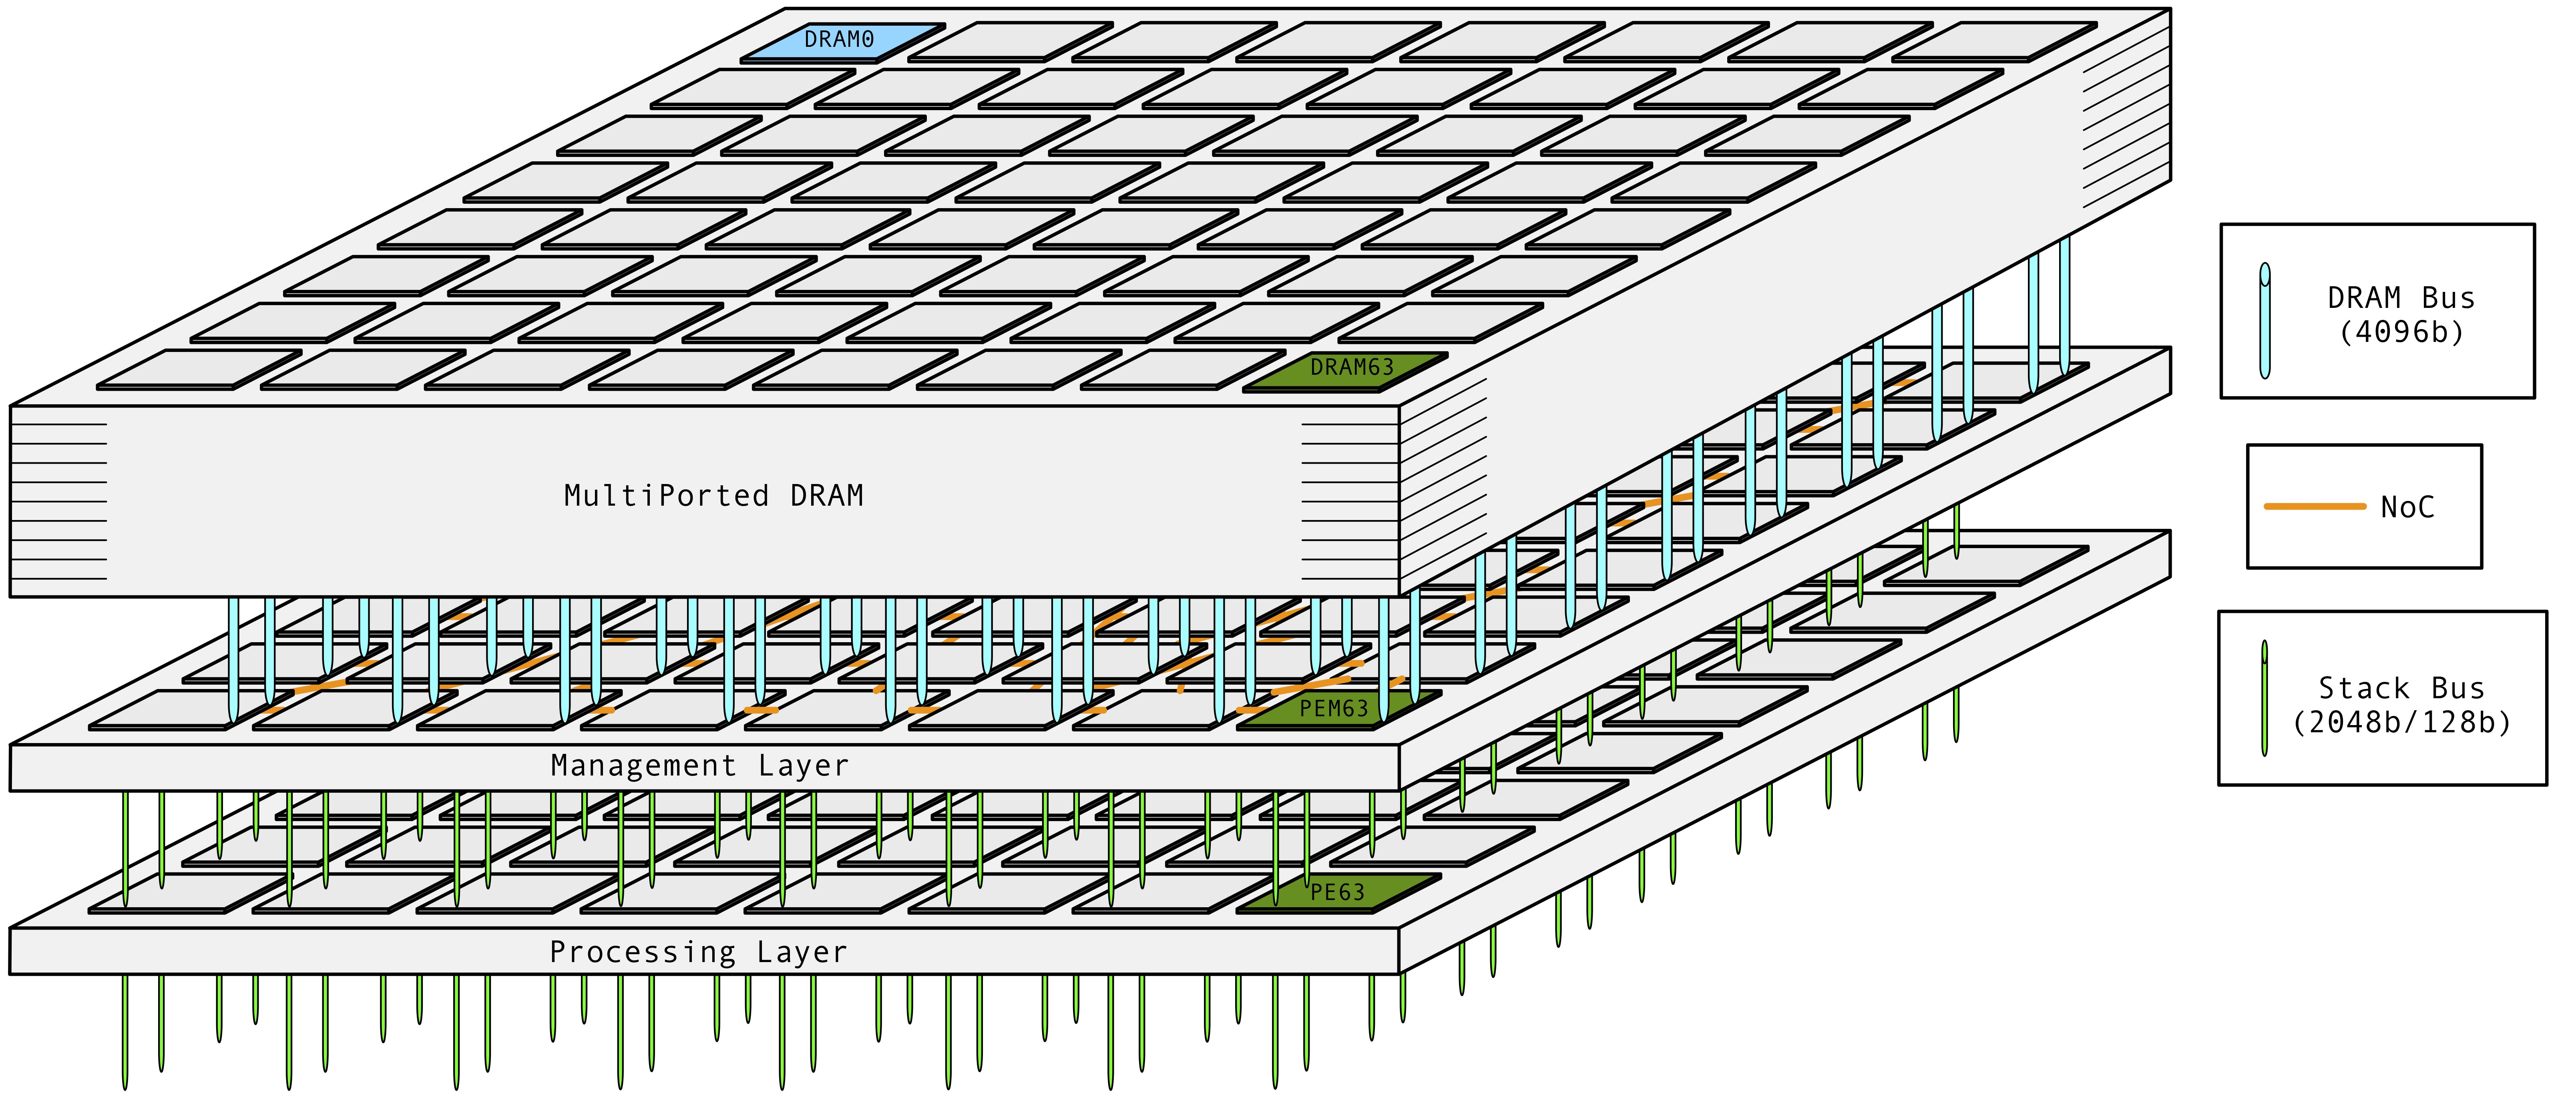
\includegraphics[width=0.9\textwidth]{SmallStackDiagram.jpg} 
        \caption{3DIC System Stack}
        \label{fig:3DICStack}
    \end{minipage}
    \hfill
    \begin{minipage}{0.3\textwidth}
        \centering
        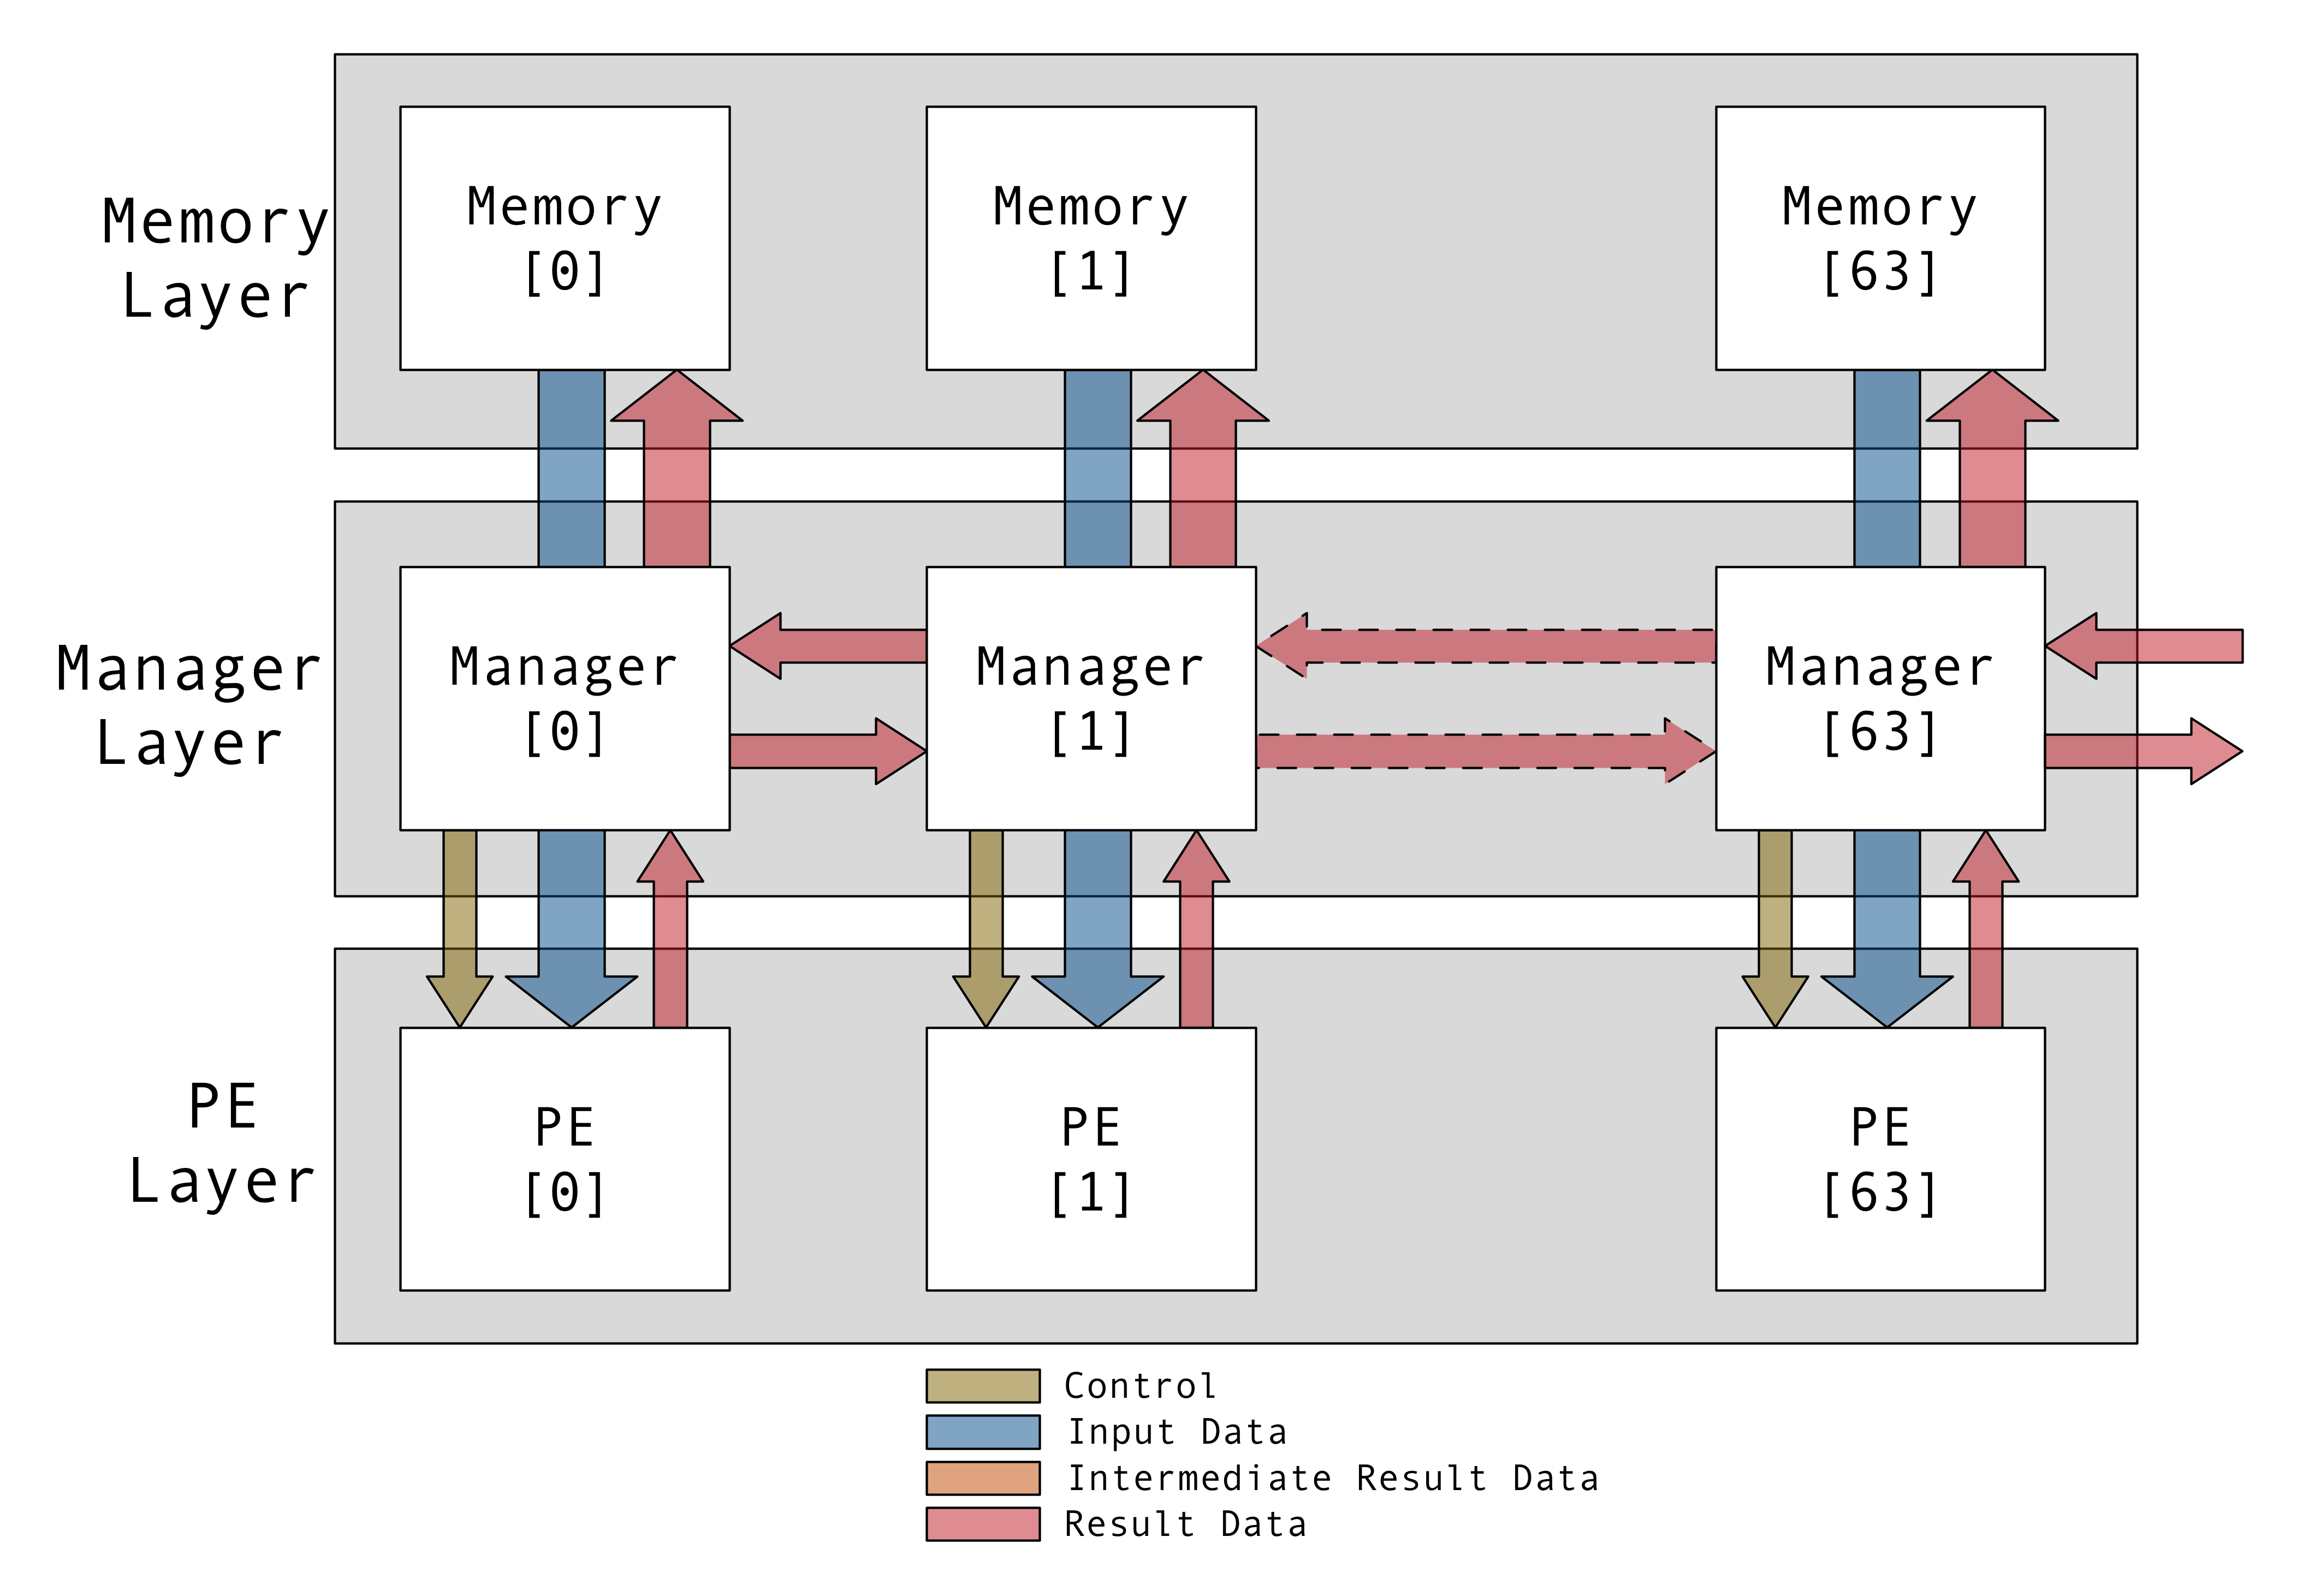
\includegraphics[width=0.9\textwidth]{FlowDiagram.jpg} 
        \caption{System showing all \ac{dram} vaults, manager and PE}
        \label{fig:FlowDiagram}
    \end{minipage}
    \hfill
    \begin{minipage}{0.3\textwidth}
        \centering
        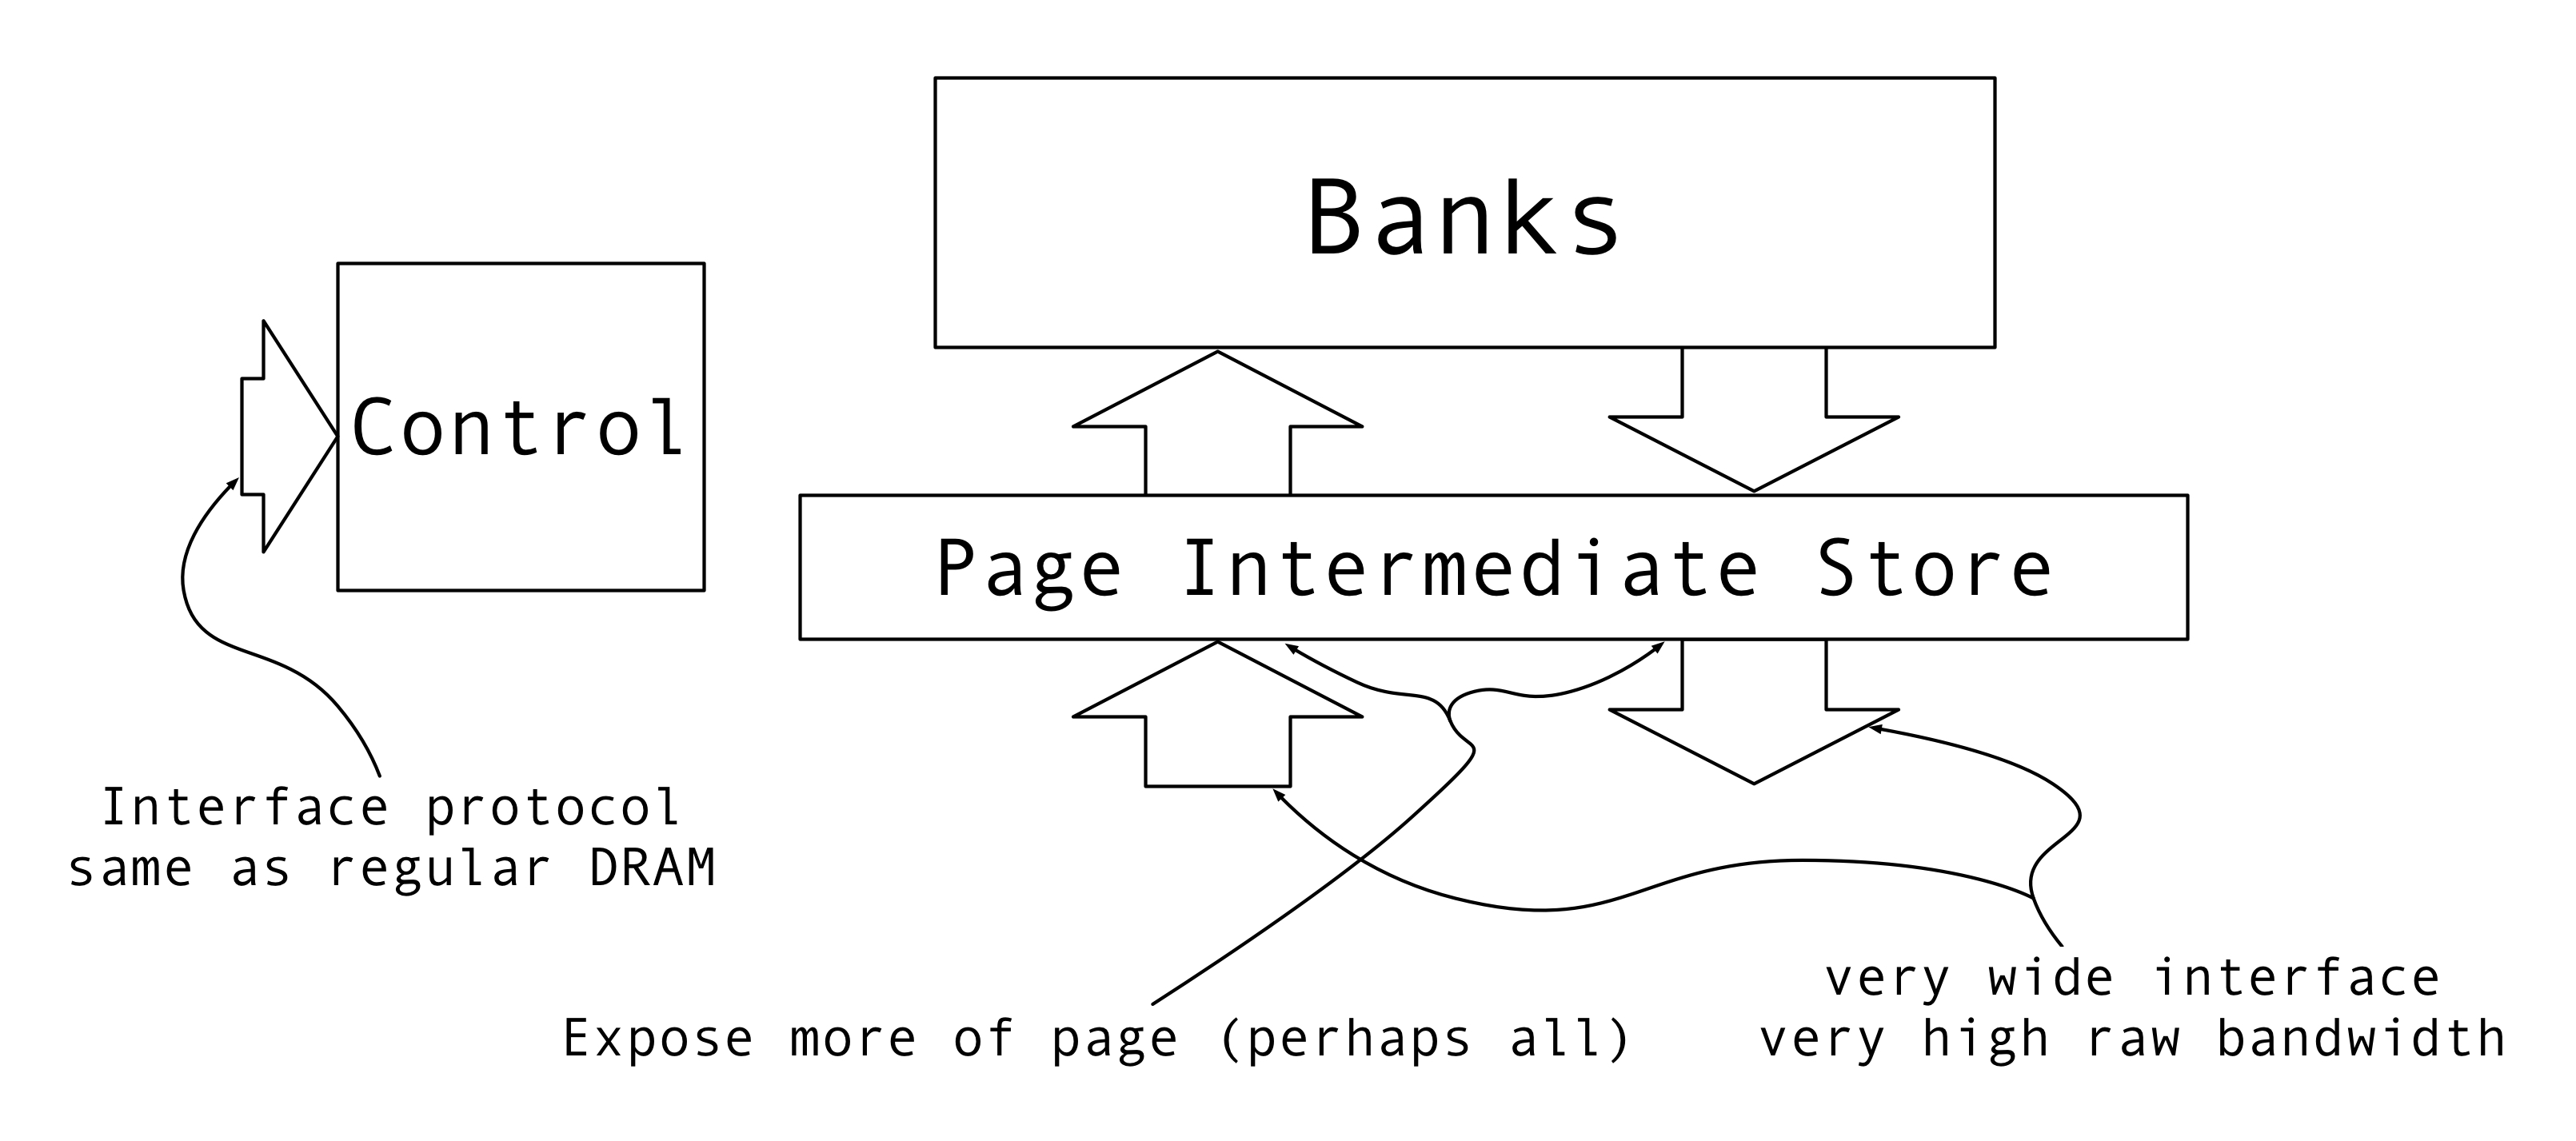
\includegraphics[width=0.9\textwidth]{DRAMBusChange.jpg} 
        \caption{DRAM WideIO Customization}
        \label{fig:customDram}
    \end{minipage}
\end{figure}
\begin{figure}[h]
    \centering
    \begin{minipage}{0.3\textwidth}
        \centering
        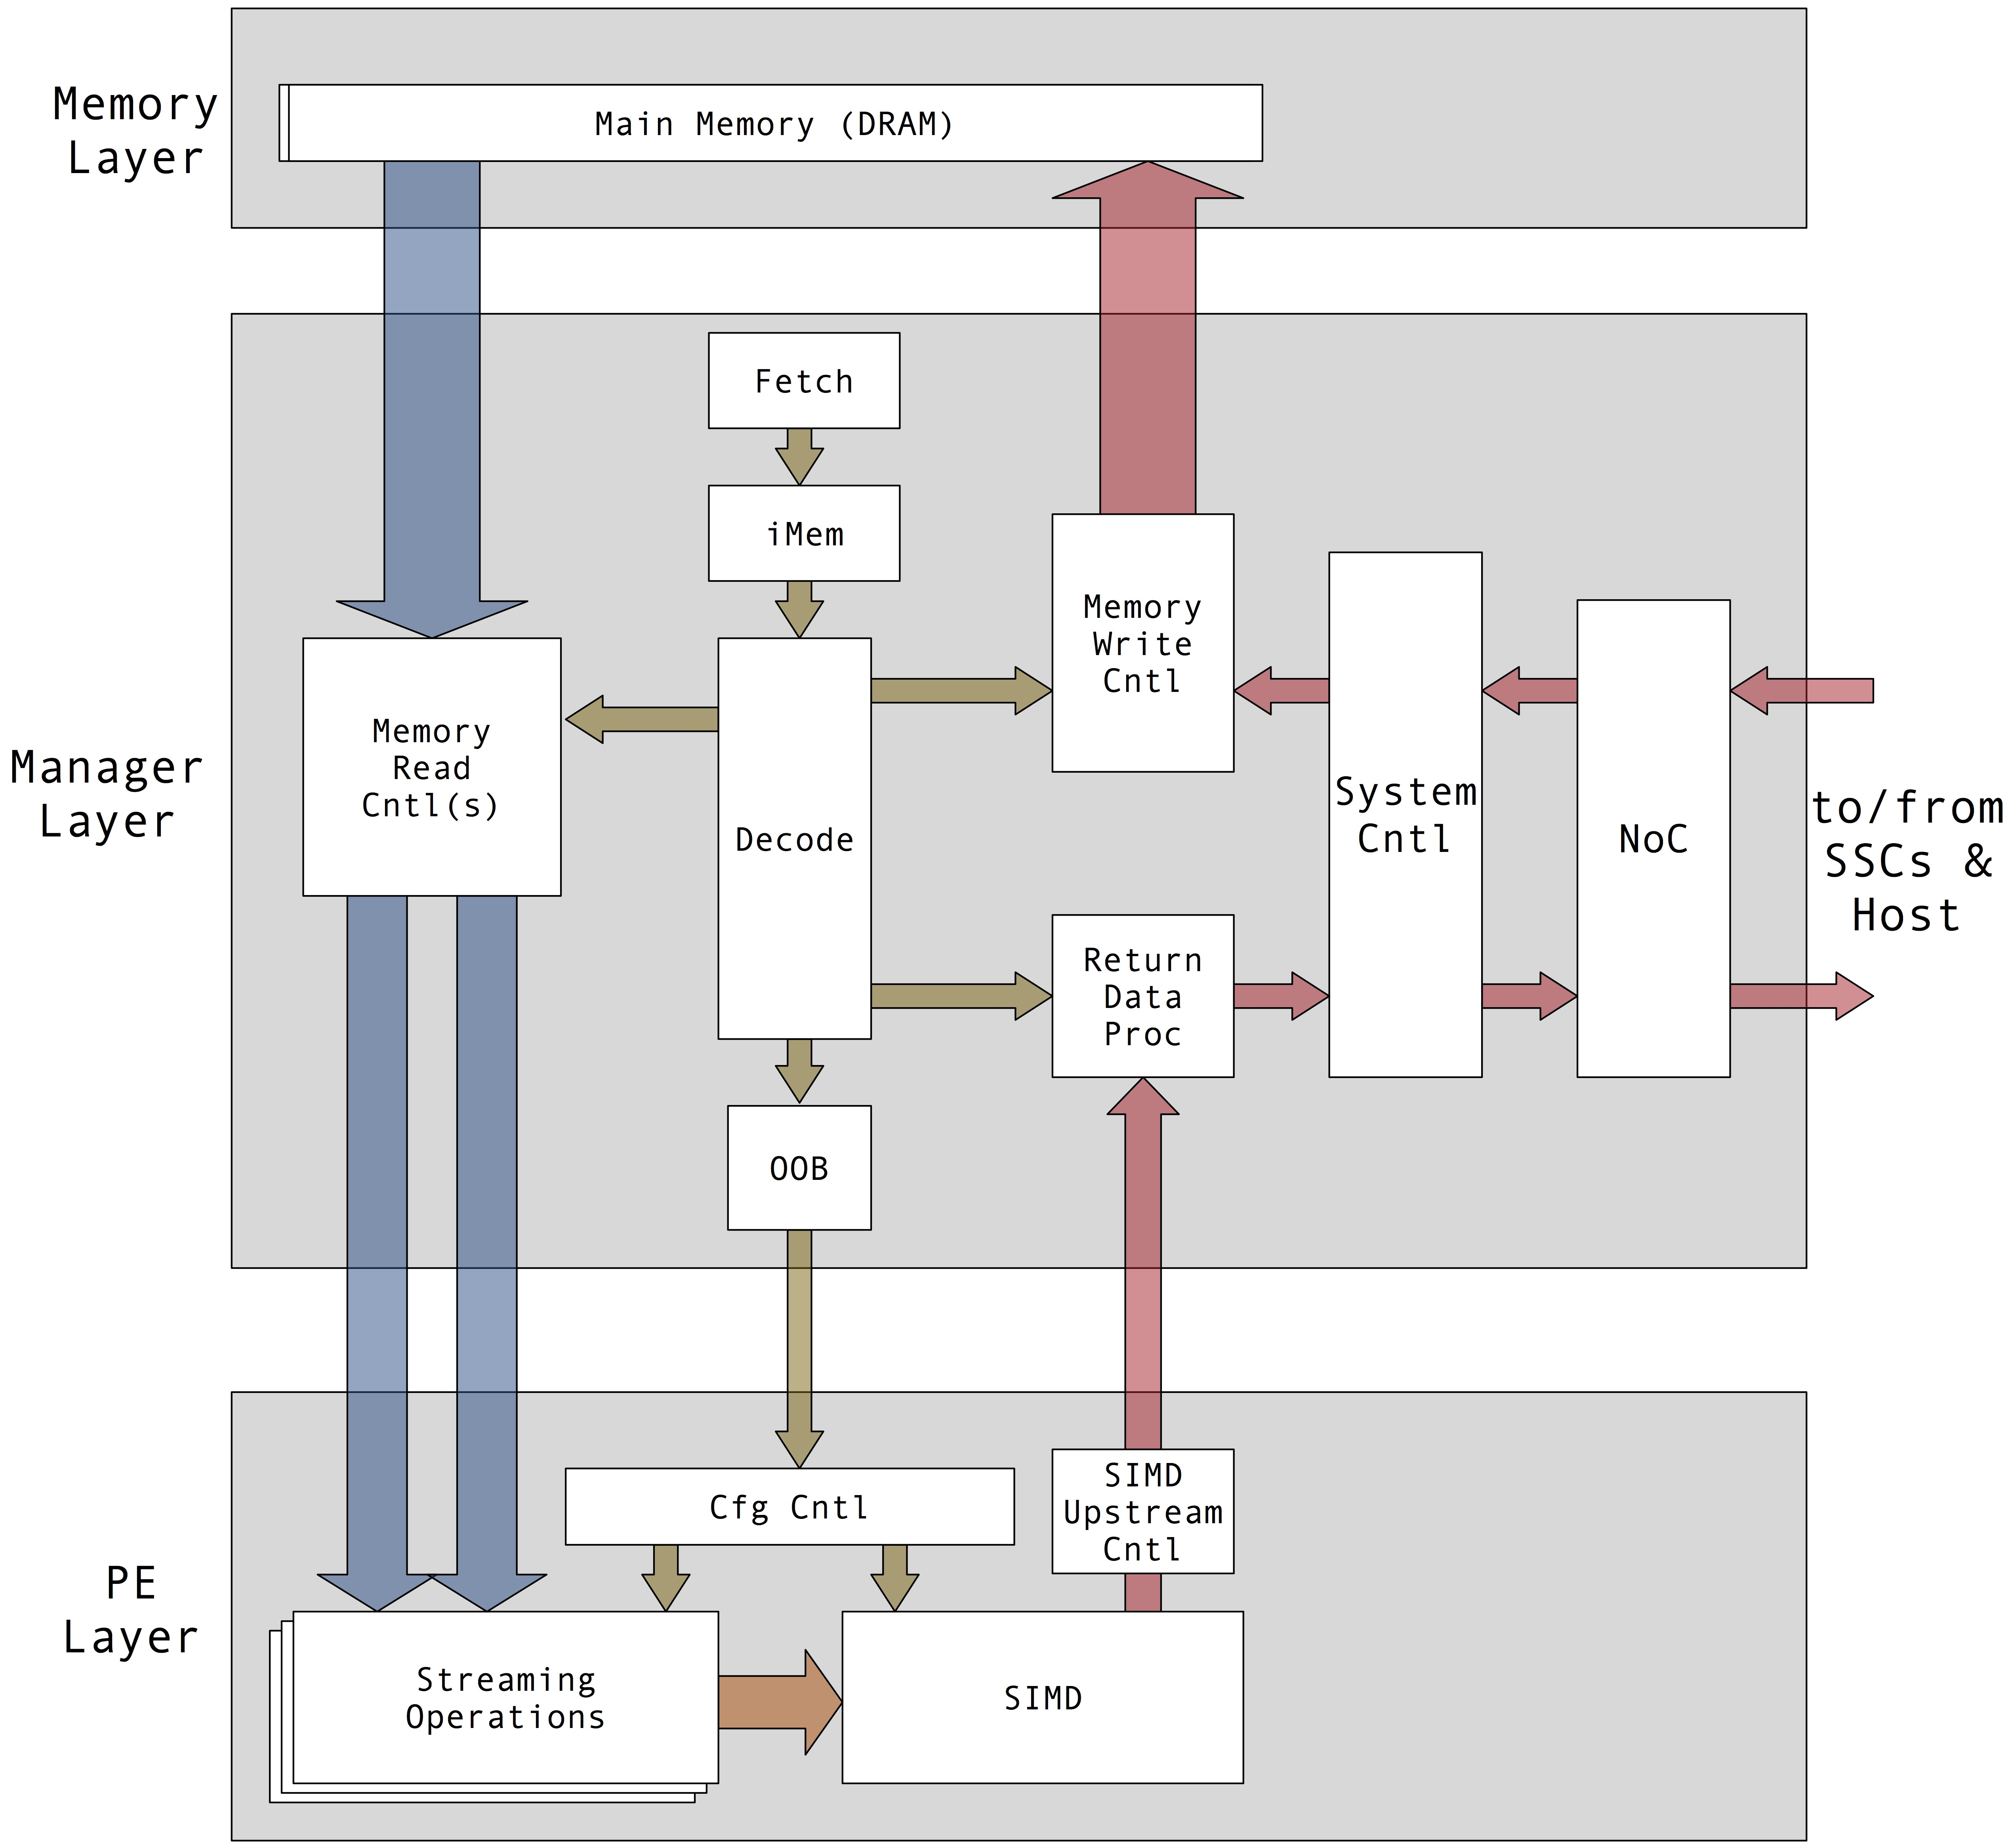
\includegraphics[width=0.9\textwidth]{DetailedFlowDiagram.jpg} 
        \caption{A single vault along with manager and PE}
        \label{fig:SSC}
    \end{minipage}
    \hfill
    \begin{minipage}{0.3\textwidth}
        \centering
        
\includegraphics[width=0.9\textwidth]{instruction4Tuple.jpg} 
        \caption{Instruction with four descriptors}
        \label{fig:instruction}
    \end{minipage}
    \hfill
    \begin{minipage}{0.3\textwidth}
        \centering
        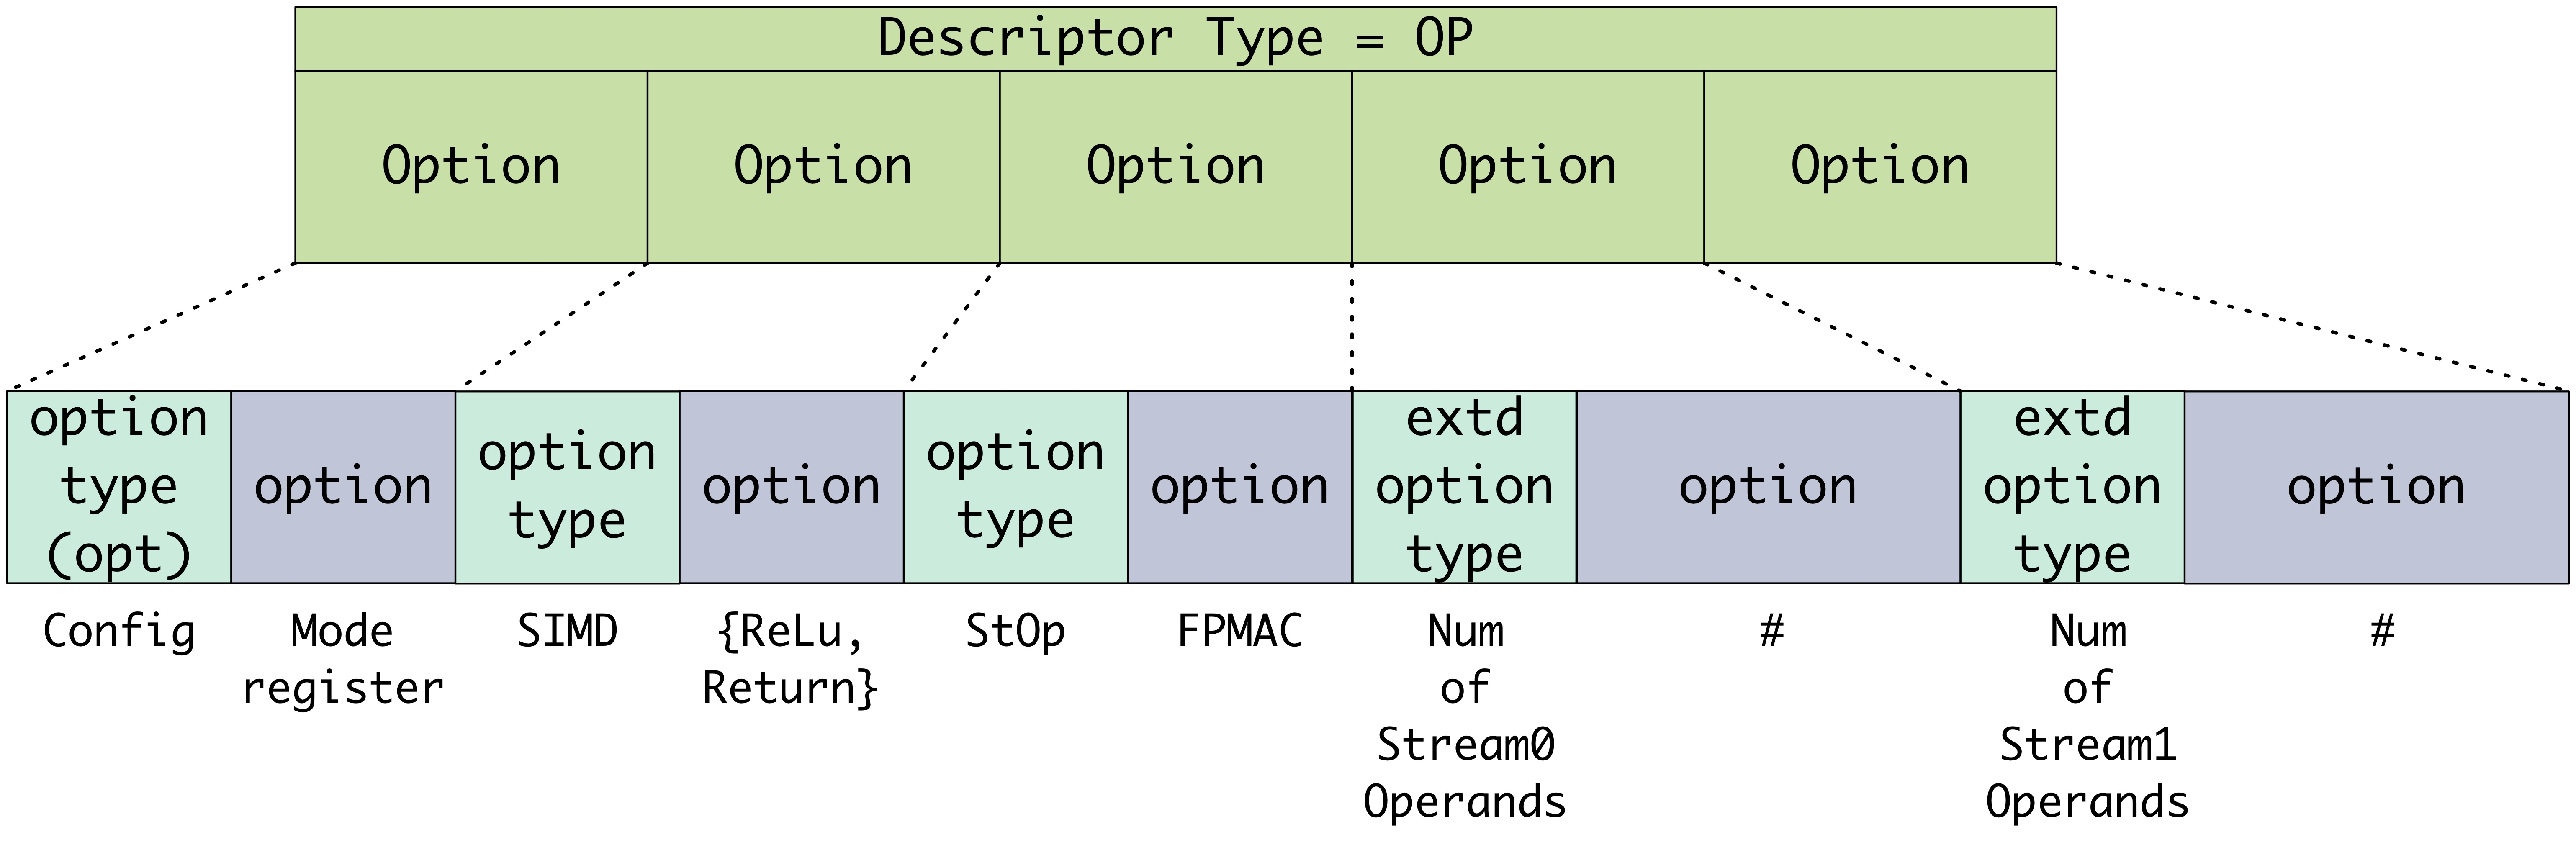
\includegraphics[width=0.9\textwidth]{descriptorTuple.jpg} 
        \caption{Descriptor with five tuples}
        \label{fig:descriptor}
    \end{minipage}
\end{figure}
\begin{figure}[h]
    \centering
    \begin{minipage}{0.3\textwidth}
        \centering
        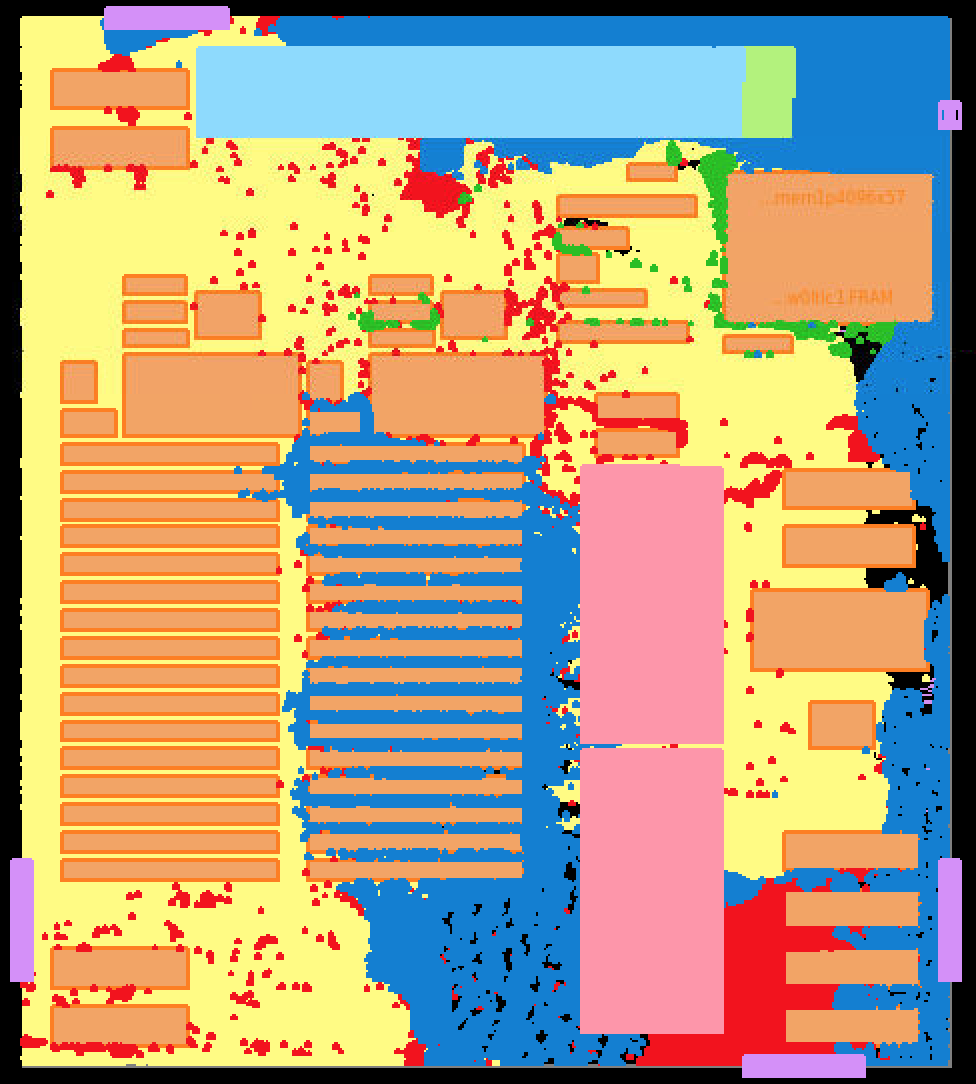
\includegraphics[width=0.9\textwidth]{ManagerLayout.png} 
        \caption{Manager Layout}
        \label{fig:managerLayout}
    \end{minipage}
    \hfill
    \begin{minipage}{0.3\textwidth}
        \centering
        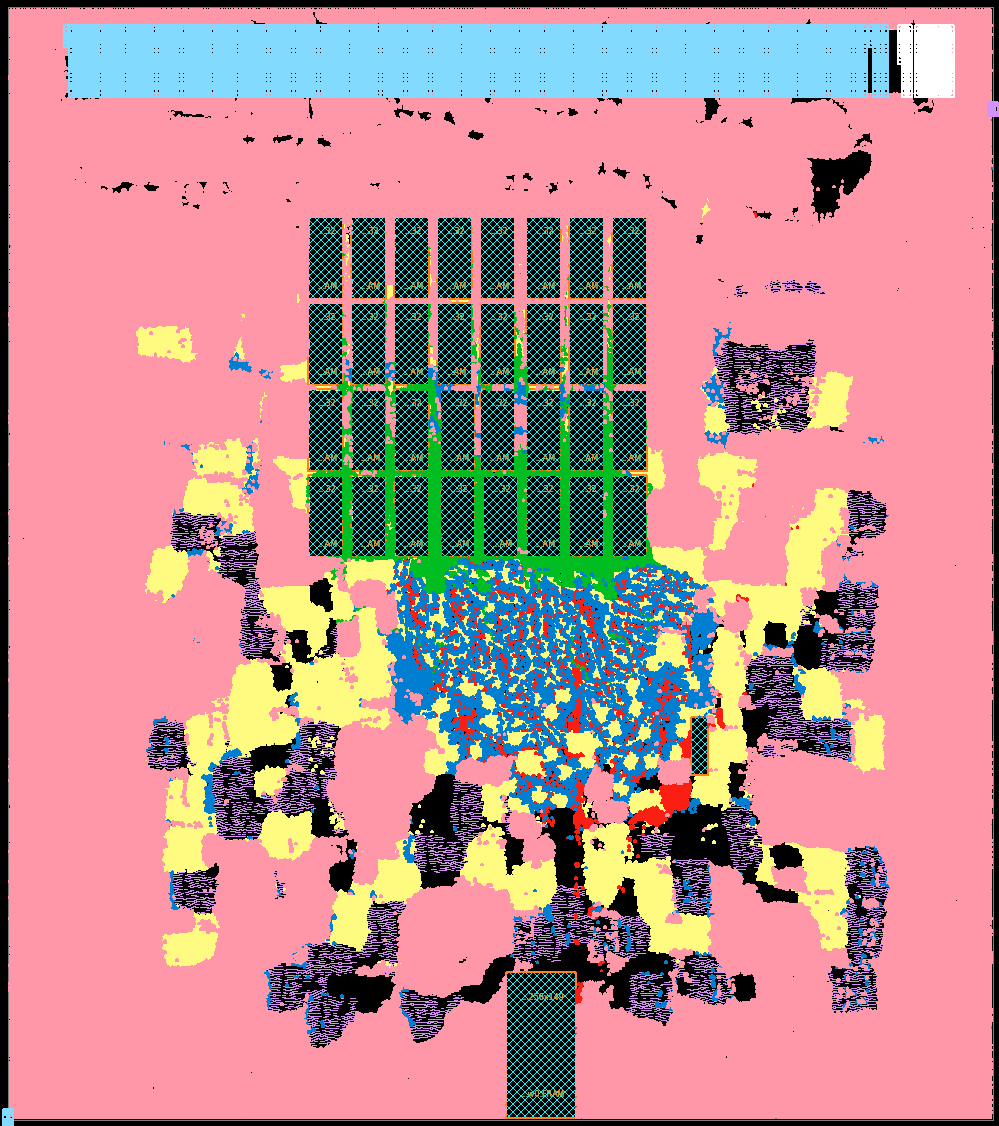
\includegraphics[width=0.9\textwidth]{PElayout.png} 
        \caption{PE Die Layout}
        \label{fig:peLayout}
    \end{minipage}
\end{figure}

%\end{abstract}

\bibliographystyle{ieeetr}
\bibliography{IEEE_3dic}

\end{document}
